  \documentclass[final,letterpaper,oneside,authoryear,11pt,singlespace,spanish]{ezthesis}
\input{Macros.tex}

\newcommand{\qed}{\nobreak \ifvmode \relax \else
      \ifdim\lastskip<1.5em \hskip-\lastskip
      \hskip1.5em plus0em minus0.5em \fi \nobreak
      \vrule height0.75em width0.5em depth0.25em\fi}

\author{Patricio Andrés Labra Medina}
\title{Simulador Laboratorio CIMUBB}
\degree{Ingeniería Civil Informática}
\supervisor{Mónica Caniupán Marileo }
\institution{Universidad del Bío-Bío, Chile}
\faculty{Facultad de Ciencias Empresariales}
\department{Departamento de Sistemas de Información}


\begin{document}
\hyphenation{com-pu-ta-dor}
\cleardoublepage
\pagenumbering{arabic}
\setcounter{page}{1}
%% En esta secci'on se describe la estructura del documento de la tesis.
%% Consulta los reglamentos de tu universidad para determinar el orden
%% y la cantidad de secciones que debes de incluir

%% # Portada de la tesis #
%% Mirar el archivo "titlepage.tex" para los detalles.

\include{titlepage}

%% # Prefacios #
%% Por cada prefacio (p.e. agradecimientos, resumen, etc.) crear
%% un nuevo archivo e incluirlo aqu'i
%% Para m'as detalles y un ejemplo mirar el archivo "gracias.tex".


\chapter*{Resumen\markboth{Resumen}{Resumen}}

La tesis tiene como objetivo abordar la necesidad identificada en el Laboratorio de Sistemas Automatizados de Producción, conocido como CIMUBB, donde se imparte formación en automatización mediante robots y computadoras. La limitación de acceso al laboratorio y la dificultad para impartir clases durante situaciones excepcionales, como la pandemia, han generado la necesidad de encontrar una solución que permita brindar enseñanza sin presencia física.

La propuesta en este informe, consiste en desarrollar un simulador en Unity, un motor de videojuegos, que reproduzca la experiencia de trabajar con los brazos robóticos Scorbot utilizados en el laboratorio. Este simulador permite a los estudiantes interactuar virtualmente con los brazos robóticos, realizando ejercicios prácticos, programación y pruebas, de manera similar a como lo harían en el laboratorio real. De esta forma, se busca preservar la calidad de la enseñanza y superar las limitaciones de acceso físico al laboratorio.

El enfoque del proyecto se basa en la recreación de los brazos robóticos Scorbot, incluyendo su funcionamiento y comportamiento. Se implementan diversas funcionalidades y herramientas que faciliten la comprensión y práctica de los conceptos de automatización, permitiendo que los estudiantes realicen actividades teóricas y prácticas desde cualquier lugar.

El resultado esperado es que este simulador se convierta en una valiosa herramienta para estudiantes y profesores del laboratorio CIMUBB, mejorando la calidad de la enseñanza en sistemas automatizados de producción y brindando la posibilidad de impartir cursos de forma virtual o complementaria a las clases presenciales.


\renewcommand{\keywords}{\textbf{\emph{Palabras Clave ---~}}}
\keywords{Simulador, Brazos Robóticos Scorbot, Unity, Sistemas Automatizados de Producción, Enseñanza Virtual, Automatización, Robótica.}

\chapter*{Abstract\markboth{Abstract}{Abstract}}

The thesis aims to address the identified need in the Automated Production Systems Laboratory, known as CIMUBB, where training in automation using robots and computers is provided. The limited access to the laboratory and the difficulty of conducting classes during exceptional situations, such as the pandemic, have created the need to find a solution that allows for teaching without physical presence.

The proposal in this report is to develop a simulator in Unity, a game engine, that replicates the experience of working with Scorbot robotic arms used in the laboratory. This simulator allows students to interact virtually with the robotic arms, performing practical exercises, programming, and tests, similar to how they would in the real laboratory. In this way, the aim is to preserve the quality of teaching and overcome the limitations of physical access to the laboratory.

The project's approach is based on the recreation of Scorbot robotic arms, including their functionality and behavior. Various features and tools are implemented to facilitate the understanding and practice of automation concepts, allowing students to engage in theoretical and practical activities from anywhere.

The expected outcome is for this simulator to become a valuable tool for students and professors at the CIMUBB laboratory, improving the quality of teaching in automated production systems and providing the possibility of conducting courses virtually or as a complement to in-person classes.

\renewcommand{\keywords}{\textbf{\emph{Keywords ---~}}}
\keywords{Simulator, Scorbot Robotic Arms, Unity, Automated Production Systems, Virtual Teaching, Automation, Robotics.}

\tableofcontents
\renewcommand{\listfigurename}{Índice de Figuras}
\listoffigures
\renewcommand{\listtablename}{Índice de Tablas}
\listoftables

\cleardoublepage

\chapter{Introducción} La pandemia de COVID-19, que comenzó a principios de 2020, tuvo un impacto significativo en diversos sectores, y la educación no fue la excepción \cite{Educacion}. Con la propagación del virus, muchas instituciones educativas se vieron obligadas a cerrar temporalmente y adoptar modalidades de enseñanza en línea para garantizar la seguridad de estudiantes y personal.

En el caso específico de la Universidad del Bío-Bío, la transición a la educación en línea generó desafíos, especialmente en disciplinas prácticas que requerían acceso a laboratorios y equipamiento especializado. El laboratorio de automatización CIMUBB, que se centra en la preparación de estudiantes para las nuevas tecnologías de automatización, se vio afectado por estas limitaciones.

El uso de robots, en este caso, los brazos robóticos SCORBOT, se vio restringido durante la cuarentena, ya que los estudiantes no podían acceder físicamente al laboratorio. Esto resultó en una disminución en la experiencia práctica y en la interacción directa con los sistemas automatizados. Los desafíos adicionales surgieron al depender de videoconferencias para la enseñanza, lo que limitó la efectividad de la instrucción práctica.

La imposibilidad de acceder al laboratorio durante la pandemia llevó al profesor Luis Vera a buscar soluciones alternativas para continuar con la enseñanza práctica. Fue en este contexto que se exploraron las tecnologías de simulación, destacando Unity como una herramienta versátil que permitiría recrear virtualmente el laboratorio de automatización CIMUBB y, específicamente, dar vida a los brazos robóticos SCORBOT.

La simulación propuesta no solo aborda la limitación impuesta por la pandemia, sino que también amplía las posibilidades de aprendizaje. Al utilizar elementos de videojuegos, se ofrece a los estudiantes la oportunidad de interactuar de manera práctica con los brazos robóticos, incluso permitiéndoles realizar experimentos y desarrollar habilidades de control directo.

Esta iniciativa representa una respuesta innovadora a los desafíos educativos presentados por la pandemia, destacando cómo las tecnologías de simulación y la creatividad pueden superar barreras físicas y brindar experiencias de aprendizaje significativas, incluso en contextos adversos como los generados por el COVID-19.

\clearpage
En este escrito, se cuenta con catorce capítulos, los cuales están ordenados de la siguiente manera:
\begin{itemize}
    \item Capitulo 1 Introducción: Este capítulo sirve como punto de partida para el trabajo, brindando una visión general del tema y su relevancia. Se establecen los objetivos de la investigación y se presenta la estructura del documento, preparando al lector para adentrarse en el análisis y exploración del tema en cuestión.
    \item Capitulo 2 Justificación: Se exponen las razones y motivos detrás de la elección de este trabajo o proyecto en particular. Se describe la importancia del tema y su relevancia en el contexto actual, destacando las problemáticas o necesidades que aborda. Ademas se presentan soluciones alternativas para el problema.
    \item Capitulo 3 Definición de la institución: Se proporciona una descripción de la institución y de la problemática a tratar.
    \item Capitulo 4 Definición de proyecto: En este capitulo se establecen los objetivos, actividades, tecnologías y herramientas para el proyecto
    \item Capitulo 5 Especificación de requerimientos de software: Se detalla el alcance que tiene el proyecto, los requerimientos y funcionalidades que el software o proyecto debe cumplir.
    \item Capitulo 6 Factibilidad: Se evalúa la viabilidad del proyecto.
    \item Capitulo 7 Análisis: Se analiza los actores que participan en el software.
    \item Capitulo 8 Diseño: Se describe el diseño del software desarrollado para resolver el problema identificado.
    \item Capitulo 9 Código: Este capitulo se presenta y explica el código desarrollado con la finalidad de darle funcionalidad al programa desarrollado.
    \item Capitulo 10 Pruebas: Se presenta las pruebas realizadas del proyecto.
    \item Capitulo 11 Plan de capacitación y entrenamiento: Se detalla el plan para capacitar.
    \item Capitulo 12 Plan de implantación y puesta en marcha: Se presenta cómo se llevará a cabo la implementación y el inicio del proyecto.
    \item Capitulo 13 Trabajos Futuros: Se analizan ideas o propuestas para futuras mejoras o expansiones del proyecto.
    \item Capitulo 14 Conclusiones: Resumen de los hallazgos, conclusiones clave y posibles recomendaciones basadas en los resultados obtenidos durante el desarrollo del proyecto.
\end{itemize}
\chapter{Justificación del Proyecto} \section{El Proyecto}
El proyecto se enfoca en abordar la necesidad de utilizar los brazos robóticos SCORBOT del laboratorio CIMUBB sin la posibilidad de acceder físicamente a ellos. Ante la situación desafiante presentada por la pandemia, la solución inicial fue el uso remoto de computadoras específicas en el laboratorio para permitir la operación a distancia de las máquinas disponibles. Esta solución fue efectiva para garantizar la continuidad de las actividades educativas y de investigación en un entorno virtual, pero presentó algunas limitaciones.

Una de las principales limitaciones es la dependencia del profesor que debe estar presente físicamente en el laboratorio para realizar el monitoreo y la supervisión de la operación remota de los brazos robóticos. Esto puede ser problemático si el profesor no puede asistir al laboratorio debido a restricciones de viaje, enfermedad u otros compromisos. La falta de presencia física puede aumentar el riesgo de fallas mecánicas o incidentes inesperados, lo que podría resultar en daños considerables en el edificio o los equipos.

La idea central de este proyecto es replicar el laboratorio CIMUBB y el funcionamiento de los brazos robóticos SCORBOT de manera virtual para abordar la necesidad de impartir conocimiento sin requerir la presencialidad física en el laboratorio. Esta solución se presenta como una alternativa efectiva y sostenible ante los desafíos planteados por la pandemia y las limitaciones para acceder a los equipos en persona.

Mediante la simulación, se crea un entorno virtual que intenta recrear fielmente el laboratorio y permite a los estudiantes y profesores interactuar con los brazos robóticos SCORBOT a distancia. Esta garantiza que el conocimiento y las habilidades prácticas relacionadas con el manejo de los brazos robóticos se puedan transmitir de manera efectiva, sin incurrir en costos adicionales de equipamiento o mantenimiento de los equipos reales. Los estudiantes pueden realizar prácticas, experimentos y proyectos de manera segura y eficiente desde sus computadoras, permitiéndoles adquirir experiencia valiosa en el uso de esta tecnología sin exponerse a riesgos físicos o daños en el edificio.

Además, la simulación ofrece una ventaja significativa al permitir la flexibilidad de horarios para los profesores y estudiantes, ya que no están limitados por las restricciones de disponibilidad del laboratorio físico. Los docentes pueden impartir clases y asesorar a los estudiantes de manera remota, brindando retroalimentación y guiándolos en sus proyectos desde cualquier lugar.

\section{Otras Soluciones}
\subsection{Robocell de Intelitek}
Intelitek es una empresa dedicada a la robótica y automatización, en su pagina dicen "brindamos a las instituciones educativas entornos interactivos de aprendizaje tecnológico". 

Uno de esos entornos es el software Robocell, un software que le agrega un entorno 3D al usuario, el el cual podrá ver un robot con dimensiones reales.
\begin{figure}[h]
\centering
\includegraphics[width=13cm]{figures/Robocell-768x588-1.jpg}
\caption{Software Robocell}
\label{fig:robocell}
\end{figure}

En la figura ~\ref{fig:robocell} se presenta la interfaz que ofrece la empresa Intelitek, esta interfaz como tal no es util, debido que el software fue desarrollado para tener una conexión al programa Scorbase.
\clearpage 

\begin{figure}[h]
\centering
\includegraphics[width=13cm]{figures/eL_RBTC_P_ScorbaseControllerUSBPro_644x350.jpg}
\caption{Software Scorbase}
\label{fig:scorbase}
\end{figure}

En la figura ~\ref{fig:scorbase} se muestra el programa Scorbase, el cual tiene como finalidad programar y operar a los brazos robóticos, además de ofrecer soporte e integración a componentes externos, por ejemplo para realizar monitoreo o cintas transportadoras.

Este programa fue creado especialmente para la operación de maquinaria física, por lo cual carece de una opción de poder visualizar el brazo robótico en uso.

\clearpage
\begin{figure}[h]
\centering
\includegraphics[width=13cm]{figures/robocell scorbase.jpg}
\caption{Software Robocell y Scorbase}
\label{fig:robobase}
\end{figure}

En la figura ~\ref{fig:robobase} se presenta ambos programas funcionando en conjunto,

\subsection{Robots Personales}

\begin{figure}[h]
\centering
\includegraphics[width=13cm]{figures/Brazo robotico.png}
\caption{Robot Arduino}
\label{fig:robotarduino}
\end{figure}

En la figura 
\chapter{Definición de la institución} En el presente capitulo se presenta la institución y el problema que se aborda en el proyecto.

\section{Descripción de la institución}
\begin{itemize}
\item Nombre: Laboratorio de Sistemas Automatizados de Producción
\item Dirección: Avenida Collao 1202, Concepción, Chile
\item Encargado: Luis Vera
\item Rubro: Automatización
\item Teléfono: (41) 311 1137
\item Descripción: Laboratorio de ensayos para el desarrollo de disciplinas en el ámbito de la Automatización Industrial, Tecnologías Avanzadas de Manufactura, Gestión de la Producción, Robótica, Control Numérico y Visión por Computador.
\end{itemize}

\section{Descripción del área de estudio}
La presente tesis tiene como objetivo principal abordar el área de estudio relacionada al laboratorio CIMUBB, el cual, por diversas razones, se puede no contar con acceso a este para realizar demostraciones prácticas. La limitación de acceso al laboratorio físico impide brindar una enseñanza completa y práctica a los estudiantes, ya que gran parte del aprendizaje depende de la interacción directa con la maquinaria y los experimentos que se encuentran en su interior.

Con el fin de superar esta limitación, se propone desarrollar un software de simulación que permita a los estudiantes experimentar y aprender de manera virtual dentro del entorno del laboratorio. El software de simulación recreará fielmente los equipos, las configuraciones y las condiciones experimentales presentes en el laboratorio real, brindando una experiencia inmersiva y cercana a la realidad.

La simulación se desarrollará utilizando tecnologías de vanguardia y siguiendo los estándares y protocolos establecidos en el campo de estudio correspondiente. Se diseñará una interfaz intuitiva y amigable para facilitar la interacción de los usuarios con los diferentes elementos del laboratorio virtual, permitiéndoles realizar experimentos, ajustar parámetros, recopilar datos y observar los resultados de sus acciones.

La creación de este software de simulación tiene como objetivo principal proporcionar una alternativa efectiva y accesible para la enseñanza y el aprendizaje en ausencia del acceso físico al laboratorio. De esta manera, se busca brindar a los estudiantes una plataforma que les permita adquirir conocimientos prácticos, desarrollar habilidades experimentales y comprender los conceptos teóricos en un entorno virtual seguro y controlado.

Se espera que esta iniciativa proporcione una solución innovadora que amplíe las posibilidades de enseñanza en el área de estudio, permitiendo a los educadores complementar las clases teóricas con experiencias prácticas simuladas. Además, se busca fomentar la autonomía y la experimentación activa por parte de los estudiantes, promoviendo el descubrimiento y la resolución de problemas dentro del contexto del laboratorio virtual.

En resumen, esta investigación se enfoca en el desarrollo de un software de simulación de laboratorio para superar la limitación de acceso físico, permitiendo así una enseñanza práctica y completa en el área de estudio correspondiente. Se espera que esta solución contribuya significativamente a la formación académica y profesional de los estudiantes, brindándoles una herramienta virtual valiosa y efectiva para su aprendizaje y desarrollo.

\section{Descripción de la problemática}
A los comienzos de la pandemia, el profesor encargado del laboratorio CIMUBB, Luis Vera, comienza a notar una necesidad para sus alumnos, necesidad que siempre estuvo presente pero, para en esa fecha, nunca había sido tan clara ni tan vital como llegó a ser.

\clearpage

\begin{figure}[h]
\centering
\includegraphics[width=10cm, height=6cm]{figures/cimubb.jpg}
\caption{Laboratorio CIMUBB}
\label{fig:cimubb}
\end{figure}

 En la Figura ~\ref{fig:cimubb} se muestra una imagen del laboratorio CIMUBB, en el cual se llevan a cabo la entrega del conocimiento sobre la automatización, para la problemática del proyecto se enfoca en los brazos robóticos SCORBOT, los cuales son tres, siendo dos modelos diferentes.\\

\begin{figure}[h]
\centering
\includegraphics[width=10cm, height=6cm]{figures/scor5p.jpg}
\caption{SCORBOT ER V Plus}
\label{fig:scor5p}
\end{figure}

 En la Figura ~\ref{fig:scor5p} se presenta el brazo robótico SCORBOT ER V Plus, es un brazo de antigua generación, teniendo cinco ejes de movimiento para el brazo robótico estático y seis ejes para el que posee una cinta de movimiento lineal.

\clearpage

\begin{figure}[h]
\centering
\includegraphics[width=10cm, height=6cm]{figures/scor9.jpg}
\caption{SCORBOT ER IX}
\label{fig:scor9}
\end{figure}

En la Figura ~\ref{fig:scor9} se presenta el brazo robótico SCORBOT ER IX, es una versión mejorada, la cual posee siete ejes de movimiento.\\

El laboratorio CIMUBB no cuenta con un entorno virtual, lo que dificulta significativamente el aprendizaje y la manipulación de los brazos robóticos SCORBOT cuando los estudiantes no pueden acceder físicamente al edificio. La falta de un entorno virtual restringe el acceso de los alumnos a prácticas y experimentos con los brazos robóticos, especialmente durante situaciones como cuarentenas, cortes de luz u otras fallas que requieren la presencia física de un supervisor o profesor.

La falta de acceso a un entorno virtual también limita la flexibilidad y disponibilidad para los estudiantes que deseen aprender sobre sistemas automatizados y brazos robóticos fuera de los horarios de clases regulares. Si el profesor no tiene acceso físico al laboratorio en un momento dado, los estudiantes se ven obligados a esperar hasta que el profesor pueda estar presente nuevamente en el lugar para realizar cualquier actividad relacionada con los brazos robóticos.
\chapter{Definición proyecto} En este capitulo se detallan los objetivos, la metodología que se utiliza, y las tecnologías en la cual se apoya.

\section{Objetivos del proyecto}

\subsection{Objetivo General}
Desarrollar una aplicación en Unity que permita simular el laboratorio
del CIMUBB, con la cual los estudiantes puedan probar el funcionamiento de los
brazos robóticos SCORBOT ER V Plus y el brazo robótico SCORBOT ER IX , intentando replicar con el mayor detalle posible
las estaciones de los brazos en el laboratorio.

\subsection{Objetivos Específicos}
\begin{enumerate}[label=\roman*.-]
\item Examinar los desafíos inherentes de la problemática que presenta el laboratorio.
\item Analizar tecnologías y herramientas con el fin de comprender su funcionamiento y utilizarlas de manera eficaz en la resolución del problema.
\item Desarrollar la aplicación.
\end{enumerate}

\subsection{Actividades}
Las actividades desarrolladas en este proyecto son:
\begin{enumerate}[label=\roman*.-]
\item Examinar los desafíos inherentes de la problemática que presenta el laboratorio.
    \begin{enumerate}[label=\arabic*.-]
    \item Investigación sobre los factores que originan la problemática.
    \end{enumerate}
\item Analizar tecnologías y herramientas con el fin de comprender su funcionamiento y utilizarlas de manera eficaz en la resolución del problema.
    \begin{enumerate}[label=\arabic*.-]
    \item Exploración y análisis de diversas herramientas de programación con el propósito de comprender sus características y funcionalidades.
    \item Investigación para evaluar las posibilidades que ofrecen distintas herramientas de programación y determinar cuál es la más adecuada para abordar el proyecto.
    \end{enumerate}
\item Desarrollar la aplicación
    \begin{enumerate}[label=\arabic*.-]
    \item Investigación sobre el laboratorio.
    \item Diseño de entorno y equipamiento.
    \item Desarrollo de código para dar funciones.
    \item Diseño de interfaz gráfica.
    \item Desarrollo de funcionalidad de la interfaz gráfica.
    \end{enumerate}
\end{enumerate}

\section{Ambiente de ingeniería de software}
\subsection{Metodología de Desarrollo}
La metodología de desarrollo a utilizar a lo largo del proyecto es incremental \cite{Incremental}, pues se debe a que facilita al desarrollo del proyecto y saber si se encuentra por un buen camino, debido a que se le presenta cada incremento al cliente y obtener una retroalimentación del mismo.

\subsection{Tecnologías}
\begin{table}[h!]
\begin{center}
\begin{tabular}{ m{0.15\linewidth} m{0.12\linewidth} m{0.65\linewidth} }
\noalign{\hrule height 2pt}
Nombre & Logo & Descripción \\ 
\noalign{\hrule height 2pt}

C\# & 
\includegraphics[height=0.12\textwidth]{figures/c.png} & 
C\# es uno de los lenguajes de programación diseñados para la infraestructura de lenguaje común . Su sintaxis básica deriva de C / C++ y utiliza el modelo de objetos de la plataforma .NET, similar al de Java, aunque incluye mejoras derivadas de otros lenguajes.
 \\
\hline
\end{tabular}
\caption{Tecnologías}
\end{center}
\end{table}

\clearpage
\subsection{Herramientas de apoyo}
\begin{table}[h!]
\begin{center}
\begin{tabular}{ m{0.15\linewidth} m{0.12\linewidth} m{0.65\linewidth} }
\noalign{\hrule height 2pt}
Nombre & Logo & Descripción \\ 
\noalign{\hrule height 2pt}

Unity & 
\includegraphics[height=0.12\textwidth]{figures/Unity.png} & 
Unity es un motor de desarrollo en tiempo real que te permite crear experiencias interactivas en el Editor de Unity que se utiliza para la creación de videojuegos. Estos se pueden publicar en diversas plataformas como PC, videoconsolas, móviles, etc. Gracias a su flexibilidad es una herramienta que también se usa en diferentes industrias como arquitectura, ingeniería, automotriz y de entretenimiento.
 \\
\hline

Blender & 
\includegraphics[height=0.09\textwidth]{figures/Blender.png} & 
Blender es un programa informático multiplataforma, dedicado especialmente al modelado, iluminación, renderizado, la animación y creación de gráficos tridimensionales. También de composición digital utilizando la técnica procesal de nodos, edición de vídeo, escultura (incluye topología dinámica) y pintura digital.
\\
\hline

Visual Studio Code & 
\includegraphics[height=0.1\textwidth]{figures/VSC.png} & 
Es un editor de código fuente desarrollado por Microsoft para Windows, Linux y macOS. Incluye soporte para la depuración, control integrado de Git, resaltado de sintaxis, finalización inteligente de código, fragmentos y refactorización de código.
\\ 
\hline

GitHub & 
\includegraphics[height=0.1\textwidth]{figures/GitHub.png} & 
Es un servicio en la nube que ayuda a los desarrolladores a almacenar y administrar su código, al igual que llevar un registro y control de cualquier cambio sobre este código.
\\ 
\hline

\end{tabular}
\caption{Herramientas de apoyo}
\end{center}
\end{table}

\chapter{Especificación de requerimientos de software} En el siguiente capitulo se presentan los requerimientos de la aplicación.

\section{Alcances}
El alcance de la simulación abarca la recreación de los brazos Scorbot y otros componentes y maquinarias presentes en el laboratorio, aunque estos últimos no serán funcionales. Entre estos elementos se incluye una cinta transportadora y un objeto específico que el brazo Scorbot podrá tomar y manipular.

La simulación se centra en replicar el comportamiento y las características de los brazos Scorbot de manera precisa, garantizando un rango de movimiento y una capacidad de manipulación de objetos lo más realista posible. Además, se incluye una representación visual detallada de los brazos Scorbot y de los demás componentes y maquinarias presentes en el laboratorio.

El brazo robótico Scorbot puede realizar su movimiento en modo Joints, el cual hace girar en función de los motores. Por otra parte, el movimiento en modo XYZ no esta disponible debido a fallos de diseño del modelado del robot. El brazo tampoco es capaz de realizar movimientos guardados, sin embargo en el código se esta planteado la lógica de esta.

La cinta transportadora esta disponible en la simulación, pero no funciona como en el entorno físico. Su presencia permite a los estudiantes experimentar con la interacción del brazo Scorbot en relación con la transferencia de objetos a lo largo de la cinta, aunque su movimiento y operación real no estarán habilitados del todo. Esto debido a darle mas importancia al brazo como tal, sin embargo, se implemento un código rustico, el cual sirve pero no esta pulido y tiene varias fallas.

Asimismo, se proporcionar un objeto específico en la simulación que el brazo Scorbot podrá tomar y manipular. Esto permite a los usuarios practicar las habilidades de agarre y manipulación del brazo, familiarizándose con los comandos y las técnicas necesarias para realizar estas tareas.

Es importante tener en cuenta que, aunque los componentes y otras maquinarias estarán presentes en la simulación, su funcionalidad real no estará activa. 

El enfoque principal será brindar a los estudiantes una experiencia interactiva y visualmente representativa del entorno del laboratorio, centrándose en la operación y el uso del brazo Scorbot. El programa no esta diseñado para personas no videntes, tampoco se contempla que el usuario no sepa usar el computador

\section{Objetivo del software}
El objetivo del software de simulación desarrollado es proporcionar una herramienta virtual que permita a los estudiantes experimentar, aprender y practicar el funcionamiento de los brazos Scorbot y otros componentes del laboratorio, en ausencia del acceso físico al mismo.

Los principales objetivos del software de simulación son:
\begin{enumerate}[label=\arabic*.-]
\item Brindar una experiencia realista: El software se diseñará con el objetivo de recrear de manera precisa y realista el comportamiento y las capacidades de los brazos Scorbot, así como otros componentes y maquinarias presentes en el laboratorio. Se buscará proporcionar una representación visual y funcionalidad detalladas, para que los estudiantes puedan interactuar con ellos de manera similar a como lo harían en el entorno físico.
\item Facilitar la práctica y el aprendizaje: El software permitirá a los estudiantes practicar y adquirir habilidades en el uso y manejo de los brazos Scorbot, así como explorar la interacción con otros componentes del laboratorio. Los usuarios podrán realizar diferentes tareas y experimentos, ajustar parámetros y recopilar datos, todo dentro de un entorno virtual controlado y seguro.
\item Fomentar la comprensión teórica y práctica: El software de simulación ayudará a los estudiantes a comprender los conceptos teóricos relacionados con el funcionamiento de los brazos Scorbot y su aplicación en diferentes situaciones. Podrán experimentar directamente los efectos de las acciones realizadas y observar los resultados de sus interacciones, lo que fortalecerá su comprensión de los principios subyacentes.
\item Superar limitaciones de acceso: Al proporcionar una alternativa virtual al laboratorio físico, el software de simulación permitirá a los estudiantes acceder al aprendizaje práctico y experiencial en cualquier momento y lugar, sin restricciones de horarios o limitaciones de espacio físico. Esto ampliará las oportunidades de aprendizaje y brindará una opción adicional para aquellos que no tienen acceso directo al laboratorio.
\end{enumerate}
\section{Descripción global del producto}
\subsection{Interfaz de usuario}
La interfaz de usuario es diseñada con un enfoque en la amigabilidad y familiaridad para minimizar la resistencia al cambio y maximizar la adaptabilidad. Al crear una interfaz que los usuarios encuentren intuitiva, se facilita su aceptación y comodidad al utilizar el software. Además, la adaptabilidad es crucial para garantizar que la interfaz funcione de manera eficiente en diferentes contextos y dispositivos, permitiendo a los usuarios acceder y utilizar el programa de manera óptima en diversas situaciones. Un diseño cuidadoso y una atención especial a la experiencia del usuario pueden fomentar una transición más fluida y exitosa hacia el software.
\subsection{Interfaz de hardware}
En el contexto de computadoras, las interfaces de hardware típicas son el teclado y el ratón para la entrada de datos, y el monitor para la salida visual. Mientras que en el caso de teléfonos y tabletas, las interfaces de hardware se basan en pantallas táctiles, que permiten a los usuarios interactuar directamente con el dispositivo mediante toques y gestos en la pantalla.
\subsection{Interfaz software}
El programa no requiere la instalación de software externo adicional, ya que funciona directamente en sistemas operativos como Windows, Linux o Android. Esto implica que los usuarios pueden ejecutar el programa sin necesidad de instalar bibliotecas o programas adicionales, lo que simplifica su implementación y uso en diferentes plataformas. La compatibilidad con estos sistemas operativos amplía la accesibilidad del programa a una variedad de dispositivos y entornos, facilitando su distribución y adopción.
\section{Requerimientos específicos}

\subsection{Requerimientos funcionales del sistema}

Se presentan los requerimientos funcionales de la aplicación, donde se destaca las características que tiene.

\begin{table}[h!]
\centering
\begin{tabular}{ | m{0.09\linewidth} | m{0.17\linewidth} | m{0.6\linewidth} | }
    \hline
    ID & Nombre & Descripción \\
    \hline
    RF-01 & Controlar el brazo robótico & La aplicación debe permitir al usuario hacer uso del brazo robótico \\
    \hline
    RF-02 & Controlar botonera & La aplicación debe permitir al usuario hacer uso de la botonera del brazo robótico \\
    \hline
\end{tabular}
\caption{Requerimientos funcionales}
\end{table}
\chapter{Factibilidad} En el capítulo actual se mostrará la factibilidad que tiene el proyecto de ser realizado.

\section{Factibilidad Técnica}

Identificar necesidades del programa y documentarlas para cumplir objetivos y satisfacer a los usuarios.

Requerimiento de uso del software en computadores:
\begin{table}[h!]
\begin{center}
\begin{tabular}{ | m{0.21\linewidth} | m{0.21\linewidth} | m{0.26\linewidth} | m{0.21\linewidth} |}
\noalign{\hrule height 2pt}
Requisitos mínimos & Windows & macOS & Linux \\ 
\noalign{\hrule height 2pt}

Versión sistema operativo & 
Windows 7 (Service Pack 1+), Windows 10 y Windows 11 & 
High Sierra 10.13+ &
Ubuntu 20.04, Ubuntu 18.04, y CentOS 7
 \\
\hline

Procesador & 
Arquitectura x86 o x64 con soporte de instrucción SSE2 & 
Arquitectura x64 con soporte de instrucción SSE2 para CPU Intel, Apple M1 o superior para CPU Apple & 
Arquitectura x64 con soporte de instrucción SSE2
 \\
\hline

API Gráfico & 
GPU compatible con DirectX versión 10, 11 o 12 & 
GPU Intel, AMD o Apple compatible con Metal &
GPU compatible con OpenGL 3.2+ o Vulkan
 \\
\hline

\end{tabular}
\caption{Requerimientos de operación computadores}
\end{center}
\end{table}

\clearpage

El programa al tener la disponibilidad de poder desarrollar una versión para celulares y derivados que posean el sistema operativo o sean capaz de ejecutar el sistema, se investiga sobre el requerimiento que se necesita en caso de ser ejecutado en alguno de estos dispositivos
\begin{table}[h!]
\begin{center}
\begin{tabular}{ | m{0.30\linewidth} | m{0.30\linewidth} | m{0.3\linewidth} |}
\noalign{\hrule height 2pt}
Requisitos mínimos & Android & iOS \\ 
\noalign{\hrule height 2pt}

Versión sistema operativo & 
Android 5.1 (API 22) & 
iOS 12
 \\
\hline

Procesador & 
ARMV7 compatible con Neon o ARM64 & 
A7 SoC
 \\
\hline

API Gráfico & 
GPU OpenGL ES 2.0 o Vulkan & 
GPU compatible con Metal
 \\
\hline

\end{tabular}
\caption{Requerimientos de operación smartphones}
\end{center}
\end{table}

Debido a que el proyecto tiene enfoque en ser utilizado en el lugar donde reside el usuario, se tomara de base los componentes que poseen los equipos que disponen en la biblioteca, pues se mantiene la idea del contexto en el cual los integrantes de la Universidad no poseen el acceso a el establecimiento, por lo cual se debía realizar el trabajo remoto desde el lugar de residencia. \\

Equipos portátiles:
\begin{itemize}
\item Procesador: Intel i3 8va gen (Por confirmar)
\item GPU: Intel HD Graphics (Por confirmar)
\item Sistema Operativo: Windows 10 (Por confirmar)
\end{itemize}

Utilizando los equipos que se encuentran disponibles en la biblioteca se puede hacer uso de la aplicación correctamente.

\section{Factibilidad Operativa}

El perfil de usuario al que va dirigido principalmente son los alumnos de la Universidad del Bío-Bío, los cuales deseen ocupar o aprender sobre el laboratorio del CIMUBB. Por otra parte, esta puede ser utilizada por cualquier persona.

\subsection{Impacto Positivo}
El impacto positivo de este proyecto es que entrega la posibilidad de poder ocupar virtualmente un laboratorio, sin necesidad de equipamiento, libre de riesgo de romper un equipo costoso.

\begin{comment}
\subsection{Impacto Negativo}
El impacto negativo es la necesidad de capacitar al usuario para el uso de los brazos robóticos, que comandos ejecutan, etc.
\end{comment}

\section{Factibilidad Económica}

Con lo visto en la factibilidad técnica, la Universidad cuenta con ordenadores que pueden ser utilizados, estos no genera gasto pero son contabilizados de igual manera.\\
\clearpage

\begin{table}[h!]
\begin{center}
\begin{tabular}{ | m{0.35\linewidth} | m{0.2\linewidth} |}
\noalign{\hrule height 2pt}
Equipamiento & Costo Por Unidad \\ 
\noalign{\hrule height 2pt}

Equipo Portátil Biblioteca & 
\$314.990
\\
\hline

\end{tabular}
\caption{Costos Equipamiento}
\end{center}
\end{table}

Para los costos del software:
\begin{itemize}
\item Unity: Se puede utilizar la versión gratuita o también la estudiante, posee versiones de pago pero no afecta el resultado.
\item Blender: Es gratuito, posee modelos ya creados de pago y gratuitos que se pueden utilizar.
\item Visual Studio Code: Es gratuito.
\item GitHub: Es gratuito, posee versiones de pago pero para el desarrollo solo influye la mejora de almacenamiento en la nube.
\end{itemize}

Para el desarrollo, al tomar el coste promedio por hora de un Ingeniero Civil Informático en Chile, el cual esta rodeando los \$6.000 por hora. Con este dato se multiplica por las horas de trabajo e investigación, las cuales en al rededor de 13 semanas, tomando en cuenta la ley chilena de no trabajar más de 45 horas a la semana, serian 585 horas en total, lo que daría unos \$3.510.000 \\
Al tomar en cuenta que se esta realizando un proyecto de título, este costo de desarrollo es despreciable. Además de que los equipos ya se encuentran disponibles, estos tampoco generan costo alguno.

\begin{table}[h!]
\begin{center}
\begin{tabular}{ | m{0.35\linewidth} | m{0.2\linewidth} |}
\noalign{\hrule height 2pt}
Variable & Costo  \\ 
\noalign{\hrule height 2pt}

Hardware & \$314.990\\

Software & 
\$0
\\
\hline

Mano de obra & 
\$3.510.000
\\
\hline

Total & 
\$3.824.990
\\
\hline

\end{tabular}
\caption{Resumen de Costos}
\end{center}
\end{table}

Se analiza los gastos que se genera por la necesidad de mantenciones a los brazos robóticos y los gastos de mantener al personal del laboratorio

\begin{table}[h!]
\begin{center}
\begin{tabular}{ | m{0.35\linewidth} | m{0.2\linewidth} |}
\noalign{\hrule height 2pt}
Variable & Costo  Mensual\\ 
\noalign{\hrule height 2pt}

Personal & 
\$1.500.000
\\

Mantención Brazo Robótico & 
\$165.000
\\
\hline

Total & 
\$1.665.000
\\
\hline

\end{tabular}
\caption{Resumen de Gasto Mensual CIMUBB}
\end{center}
\end{table}

Al tener en cuenta la finalidad del proyecto, el cual no busca reemplazar el laboratorio como tal, sino dar una alternativa para poder acceder a la simulación del laboratorio desde el lugar de residencia, se podría reducir las horas de trabajo del personal del laboratorio, el cual trabaja 45 horas a la semana, al contar el mes como cuatro semanas, se obtiene que semanalmente es un gasto de \$375.000. Al ser 45 horas, y contando la semana desde lunes a viernes, el personal trabaja 9 horas diarias, por lo cual diariamente se tiene un gasto de \$75.000. Con esto se analiza que:

\begin{figure}[h]
\centering
    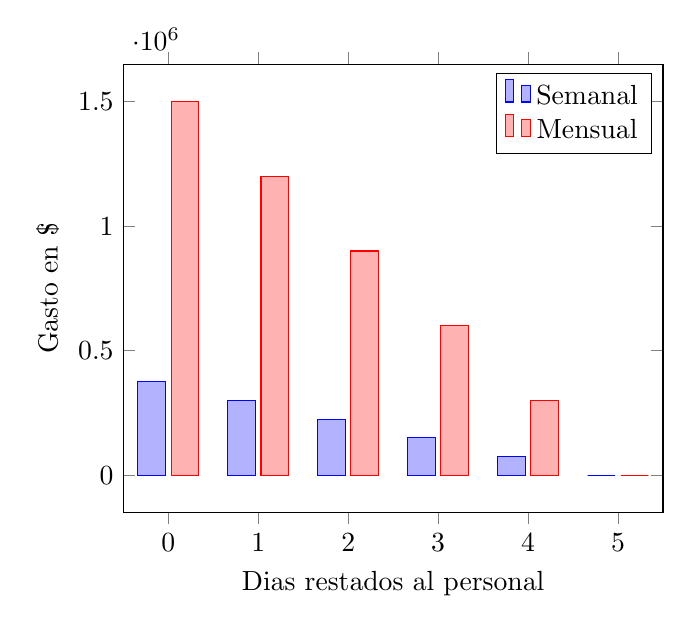
\begin{tikzpicture}
        \begin{axis}[ybar , ylabel={Gasto en \$} , xlabel={Dias restados al personal}]
        \addplot+ [draw = blue] coordinates{
        (0,375000) 
        (1,300000)
        (2,225000)
        (3,150000)
        (4,75000)
        (5,0)
        };
        \addplot+ [draw = red] coordinates{
        (0,1500000) 
        (1,1200000)
        (2,900000)
        (3,600000)
        (4,300000)
        (5,0)
        };
        \legend {Semanal, Mensual}
        \end{axis}
    \end{tikzpicture}
\caption{Análisis gasto Personal CIMUBB}
\label{gasto}
\end{figure}

En la Figura ~\ref{gasto} se logra apreciar la reducción de gasto al reducir los días de trabajo del personal. Sin embargo, para las mantenciones no se pueden reducir, estas son contabilizadas anualmente y son de manera correctiva y no preventiva, siendo esta necesaria por el mal uso de los usuarios y nunca por el desgasto natural.  
\section{Conclusión de la factibilidad}
En cuanto a la factibilidad técnica, la universidad dispone de las herramientas necesarias para el desarrollo y para su uso, se puede llegar a realizar y ocupar sin tener mayores gastos. \\
Por otra parte, al revisar los gastos mensuales, se llega a concluir que la aplicación reduciría un gasto considerable.
\chapter{Análisis} En este capitulo que nos conlleva a analizar los actores que ejecutaran la aplicación, los flujos que esta tendrá.

\section{Procesos de negocios futuros}
\begin{figure}[h]
\centering
\includegraphics[height=6.83cm]{figures/bpmn.png}
\caption{Modelo y Notación de Procesos de Negocio}
\label{fig:bpmn}
\end{figure}

En la Figura 7.1 se muestra el proceso de como el usuario interactúa con la simulación, el proceso inicia con el usuario ejecutando la simulación, una vez dentro de esta, el usuario puede elegir entre usar el brazo robótico, cambiar de brazo robótico, con las cuales lo lleva a mantenerse en el proceso de la simulación, por ultimo esta la opción de salir de la simulación que finaliza este proceso

\section{Casos de uso}
\subsection{Actores}
Usuario: Persona que utilizara la aplicación, ya sea estudiante o profesor de la Universidad del Bío-Bío, como también personas externas a esta. El usuario puede utilizar la aplicación completamente.
\subsection{Diagrama de casos de uso y descripción}

\begin{figure}[h]
\centering
\includegraphics[height=6.83cm]{figures/usuario.png}
\caption{Diagrama de caso de uso: Usuario}
\label{fig:usuario}
\end{figure}

Como se logra apreciar en la Figura ~\ref{fig:usuario}, se muestran las interacciones que tiene el usuario en la aplicación. El actor es simplemente un usuario, ya que la aplicación es de uso personal.

\subsection{Especificación de los caso de uso}

\begin{table}[h!]
\begin{center}
\begin{tabular}{| m{0.19\linewidth} | m{0.75\linewidth} |}
\hline
\multicolumn{2}{ |c| }{Caso de Uso: Visualizar control de brazo robot} \\ \hline
ID & CU-01 \\ \hline
Descripción & El actor puede visualizar el control de brazo robot. \\ \hline
Actores & Usuario \\ \hline
Flujo principal & 

\begin{enumerate}[label=\arabic*.-]
    \item El actor debe haberse dirigido al menú desplegable
    \item El actor debe seleccionar la opción de "Visualizar Control"
\end{enumerate}

\\ \hline
\end{tabular}
\caption{Especificación de casos de uso: Visualizar control de brazo robot}
\end{center}
\end{table}

\begin{table}[h!]
\begin{center}
\begin{tabular}{| m{0.19\linewidth} | m{0.75\linewidth} |}
\hline
\multicolumn{2}{ |c| }{Caso de Uso: Manejar control de brazo robot} \\ \hline
ID & CU-02 \\ \hline
Descripción & El actor puede manejar el control de brazo robot. \\ \hline
Actores & Usuario \\ \hline
Flujo principal & 

\begin{enumerate}[label=\arabic*.-]
    \item El actor debe haberse dirigido al menú desplegable
    \item El actor debe seleccionar la opción de "Visualizar control de brazo robot"
\end{enumerate}

\\ \hline
\end{tabular}
\caption{Especificación de casos de uso: Manejar control de brazo robot}
\end{center}
\end{table}

\begin{table}[h!]
\begin{center}
\begin{tabular}{| m{0.19\linewidth} | m{0.75\linewidth} |}
\hline
\multicolumn{2}{ |c| }{Caso de Uso: Visualizar brazo robot} \\ \hline
ID & CU-03 \\ \hline
Descripción & El actor puede visualizar el brazo robot. \\ \hline
Actores & Usuario \\ \hline
Flujo principal & 

\begin{enumerate}[label=\arabic*.-]
    \item El actor debe haber abierto la aplicación
\end{enumerate}

\\ \hline
\end{tabular}
\caption{Especificación de casos de uso: Visualizar brazo robot}
\end{center}
\end{table}

\begin{table}[h!]
\begin{center}
\begin{tabular}{| m{0.19\linewidth} | m{0.75\linewidth} |}
\hline
\multicolumn{2}{ |c| }{Caso de Uso: Controlar brazo robot} \\ \hline
ID & CU-04 \\ \hline
Descripción & El actor puede controlar el brazo robot. \\ \hline
Actores & Usuario \\ \hline
Flujo principal & 

\begin{enumerate}[label=\arabic*.-]
    \item El actor debe haberse dirigido al menú desplegable
    \item El actor debe seleccionar el robot a utilizar
    \item El actor controla a través de teclado el robot
\end{enumerate}

\\ \hline
\end{tabular}
\caption{Especificación de casos de uso: Controlar brazo robot}
\end{center}
\end{table}
\chapter{Diseño} En este capítulo, se presenta el diseño de interfaz de la aplicación desarrollada, y las diferentes opciones que se presentan.
\section{Diseño interfaz y navegación}

En la Figura \ref{fig:Mockup} se presenta un bosquejo de la interfaz del usuario, la cual muestra la simulación principalmente, y además un control flotante. También se muestran los menús desplegables.
\begin{figure}[ht]
\centering
\includegraphics[width=16cm]{figures/Mockup.png}
\caption{Mockup}
\label{fig:Mockup}
\end{figure}
\clearpage

\begin{figure}[ht]
\centering
\includegraphics[width=16cm]{figures/menu.png}
\caption{Menu Principal Simulación}
\label{fig:menu}
\end{figure}

Las distintas opciones que se muestran en la Figura ~\ref{fig:menu} se detallaran a continuación
\begin{itemize}
\item Entrar: Permite entrar a la simulación.
\item Reiniciar: Permite reiniciar la simulación, volviendo a la posición original.
\item Resolución: Permite cambiar la resolución del programa, esto permite adaptarse a diferentes resoluciones o utilizar menos recursos.
\item Calidad Imagen: Permite cambiar la calidad visual de la simulación, esto permite adaptarse a cualquier equipo ya tenga buenos recursos o no.
\item Pantalla Completa: Permite que el programa funcione en pantalla completa o en modo ventana,
\item Salir: Permite salir de la aplicación.
\end{itemize}

\clearpage
\begin{figure}[ht]
\centering
\includegraphics[width=16cm]{figures/simulacion.png}
\caption{Interfaz dentro de la Simulación}
\label{fig:interfaz}
\end{figure}


Las distintas opciones que se muestran en la Figura ~\ref{fig:interfaz} se detallaran a continuación
\begin{itemize}
\item Pausar: Permite pausar la simulación y volver al menu.
\item Lista Cámaras: Permite cambiar la perspectiva del usuario.
\item Lista Brazos Robóticos: Permite cambiar al robot controlado por el usuario.
\item Interruptor Mostrar Control: Permite cambiar la visibilidad de la botonera.
\item Interruptor Activar Cinta: Permite cambiar el estado de la cinta transportadora.
\item Botonera: Realiza las operaciones replicando el control de los brazos Scorbot reales.
\end{itemize}
\chapter{Código} En este capitulo, se presenta explicaciones sobre el código fuente de la aplicación desarrollada.
\section{Lógica Cinta Transportadora} 
\lstset{language=[Sharp]C, breaklines=true, basicstyle=\footnotesize}
\begin{lstlisting}[frame=single]
using System;
using System.Collections;
using System.Collections.Generic;
using UnityEngine;

public class Belt : MonoBehaviour
{
    public float speed =5f;
    Rigidbody rBody;
    public Vector3 direccion;

    void Start()
    {
        rBody = GetComponent<Rigidbody>();
    }

    void FixedUpdate()
    {
        Vector3 pos = rBody.position;
        rBody.position += direccion * speed * Time.fixedDeltaTime;
        rBody.MovePosition(pos);
    }
}
\end{lstlisting}
Este código proporciona la lógica simple de movimiento de objetos en la cinta transportadora, sin embargo este no llega a replicar su funcionamiento real debido a limitaciones que se explica en los detalles siguientes:

\begin{lstlisting}[frame=single]
using System;
using System.Collections;
using System.Collections.Generic;
using UnityEngine;
\end{lstlisting}
Estas líneas son declaraciones de uso de espacio de nombres (namespace) que indican qué bibliotecas se están utilizando en el código. Están importando las bibliotecas necesarias para trabajar con Unity y otros espacios de nombres estándar de C\#.

\begin{lstlisting}[frame=single]
public class Belt : MonoBehaviour
{
    ...
}
\end{lstlisting}
Aquí comienza la definición de la clase Belt, que hereda de la clase MonoBehaviour. Esto significa que este script puede ser adjuntado a objetos en Unity y ejecutado como parte del comportamiento de esos objetos.

\begin{lstlisting}[frame=single]
    public float speed =5f;
    Rigidbody rBody;
    public Vector3 direccion;
\end{lstlisting}
En esta parte se declaran las variables, se parte con una variable pública llamada speed (velocidad) que tiene un valor predeterminado de 5. Esta variable representa la velocidad a la que se moverá la cinta transportadora.
Después se declara una variable llamada rBody de tipo Rigidbody. Esta variable se utilizará para almacenar una referencia al componente Rigidbody adjunto al objeto al que se adjunte este script. Un Rigidbody es un componente utilizado en el desarrollo de videojuegos y simulaciones físicas para representar objetos que tienen propiedades físicas, como masa, velocidad, y fuerzas que actúan sobre ellos.
Por ultimo se declara una variable pública llamada direccion (dirección) de tipo Vector3. Vector3 es una estructura de datos utilizada para representar vectores tridimensionales en un espacio tridimensional. Esta variable se utiliza para definir la dirección en la que se moverá la cinta transportadora. La dirección se establece desde el Inspector de Unity cuando adjuntes este script a un objeto en el juego.

\begin{lstlisting}[frame=single]
    void Start()
    {
        rBody = GetComponent<Rigidbody>();
    }
\end{lstlisting}
El método Start() es uno de los métodos especiales en Unity que se llama automáticamente cuando se inicia un objeto al que se adjunta un script, en este caso se obtiene una referencia al componente Rigidbody del objeto al que se adjunta este script. Esto se hace utilizando la función GetComponent<Rigidbody>(), y la referencia se almacena en la variable rBody.
\clearpage
\begin{lstlisting}[frame=single]
    void FixedUpdate()
    {
        ...
    }
\end{lstlisting}
FixedUpdate es un método especial que se encuentra en Unity y es utilizado para realizar cálculos y actualizaciones relacionadas con la física en un juego. A diferencia de Update, que se llama una vez por cada fotograma (frame) renderizado, FixedUpdate se llama en intervalos de tiempo fijos y regulares, lo que lo hace especialmente adecuado para manejar la simulación de física y movimiento en un juego.

\begin{lstlisting}[frame=single]
        Vector3 pos = rBody.position;
\end{lstlisting}
Aquí se crea una variable local llamada pos que almacena la posición actual del objeto asociado al Rigidbody.

\begin{lstlisting}[frame=single]
        rBody.position += direccion * speed * Time.fixedDeltaTime;
\end{lstlisting}
Esta línea actualiza la posición del objeto con el componente Rigidbody (rBody) al agregarle un desplazamiento basado en la dirección (direccion), la velocidad (speed), y el tiempo transcurrido (Time.fixedDeltaTime). Esto aun no simula el movimiento de la cinta transportadora y se explica con las siguientes figuras. 
\begin{figure}[h]
\centering
\includegraphics[width=10cm, height=6cm]{figures/rbodyposition1.png}
\caption{rigidBody Position 1}
\label{fig:rbodyposition1}
\end{figure}


En la Figura ~\ref{fig:rbodyposition1} se presenta el movimiento de la cinta, este movimiento solo aplica para la cinta, a diferencia del método MovePosition que se presenta más adelante.
\clearpage

\begin{figure}[h]
\centering
\includegraphics[width=10cm, height=6cm]{figures/rbodyposition2.png}
\caption{rigidBody Position 2}
\label{fig:rbodyposition2}
\end{figure}

En la Figura ~\ref{fig:rbodyposition2} se muestra donde finaliza el movimiento, como se aprecia este solo mueve la cinta y el objeto sobre esta no posee movimiento

\begin{lstlisting}[frame=single]
        rBody.MovePosition(pos);
\end{lstlisting}
En este método, se devuelve la cinta a su posición original, la diferencia que con el método de movimiento anterior es que si se mueve el objeto, tal como se presenta en las siguientes figuras.
\begin{figure}[h]
\centering
\includegraphics[width=10cm, height=6cm]{figures/rbodymove1.png}
\caption{rigidBody MovePosition 1}
\label{fig:rbodymove1}
\end{figure}

En la Figura ~\ref{fig:rbodymove1} se presenta el movimiento de la cinta, este movimiento aplica tanto para la cinta como para el objeto.

\clearpage

\begin{figure}[h]
\centering
\includegraphics[width=10cm, height=6cm]{figures/rbodymove2.png}
\caption{rigidBody MovePosition 2}
\label{fig:rbodymove2}
\end{figure}

En la Figura ~\ref{fig:rbodymove2} se muestra donde finaliza el movimiento, como se aprecia este mueve tanto la cinta y como el objeto.

Con esta sucesión de movimientos, la cinta al "ir para atrás" sin mover el objeto, y después "volver a su posición" moviendo el objeto, repitiéndolo una y otra vez se logra el efecto de una cinta transportadora. El problema es que el objeto solo se mueve y en las esquinas no rota como en el laboratorio.
\clearpage
\section{Lógica Brazos Robóticos}
Para esta lógica, se explican los detalles mas importantes debido a que el código es demasiado extenso.
\begin{lstlisting}[frame=single]
   //Base
    public float velocidadRotacionBase = 50.0f; // Velocidad de rotacion
    public KeyCode teclaRotacionPositivaBase = KeyCode.Q; // Tecla para la rotacion en direccion positiva
    public KeyCode teclaRotacionNegativaBase = KeyCode.A; // Tecla para la rotacion en direccion negativa
    public Transform Base; // Transform del objeto que se va a rotar
    private float LimitePositivoBase = 155.0f; // Angulo limite del objeto
    private float LimiteNegativoBase = -155.0f; // Angulo limite del objeto
    private float sumaRotacionBase = 0.0f; // Suma de la rotacion del objeto para su uso en limites

    //Shoulder
    public float velocidadRotacionShoulder = 50.0f; // Velocidad de rotacion
    public KeyCode teclaRotacionPositivaShoulder = KeyCode.W; // Tecla para la rotacion en direccion positiva
    public KeyCode teclaRotacionNegativaShoulder = KeyCode.S; // Tecla para la rotacion en direccion negativa
    public Transform Shoulder; // Transform del objeto a rotar
    public Transform puntoFijoShoulder; // Transform del punto fijo alrededor del cual se realizara la rotacion
    private float LimitePositivoShoulder = 10.0f; // Angulo limite del objeto
    private float LimiteNegativoShoulder = -130.0f; // Angulo limite del objeto
    private float sumaRotacionShoulder = 0.0f; // Suma de la rotacion del objeto para su uso en limites
\end{lstlisting}
Para explicar las declaraciones de las partes de los brazos, se toma en cuenta dos partes distintas pero aplica para cualquier otra parte similar, la base es un objeto que tiene rotación sobre su propio eje, es decir no necesita otro punto para rotar o rota sobre su propio centro, a diferencia del Shoulder o un brazo cualquiera, para rotar este tiene un punto fijo en uno de sus extremos y no en el centro.
Se empieza con declarar la velocidad de la rotación del objeto en una variable float. Después se declaran variables tipo KeyCode que sirven para almacenar la información de una tecla en el teclado en particular, esto se realiza para realizar pruebas de movimiento.
Al declarar una variable de tipo Transform, en Unity, un "Transform" se refiere a un componente fundamental que se encuentra en la mayoría de los objetos en un escenario 3D o 2D. El componente Transform está asociado con la posición, rotación y escala de un objeto en el espacio de juego. Básicamente, controla la ubicación y la orientación de un objeto en el mundo virtual creado en Unity. Con esta variable se puede guardar toda la información previamente descrita, con la finalidad de realizar movimientos. En casos de rotación sobre el mismo objeto como la Base, solo se pide una variable, para objetos con centro en su extremo se piden dos variables, mas adelante se detallara como funciona el movimiento y el motivo de pedir uno o dos variables.
Y por ultimo se tienen los limites, consisten en dos variables que marcan el limite de operación de cada parte, para este caso se utilizan los limites establecidos mecánicamente por la misma unidad descrita en su manual. Y también la suma de rotación, la cual almacenara como tal el movimiento realizado, esto para ser utilizado en la comprobación de limites

\begin{lstlisting}[frame=single]
    private string nombreObjeto = "";
\end{lstlisting}
En esta linea se declara una variable para identificar la parte que se moverá con la botonera.

\begin{lstlisting}[frame=single]
    private bool positivoboton = false;
    private bool negativoboton = false;
\end{lstlisting}
Con estas variables sirven para saber si el botón presionado es positivo o negativo

\begin{lstlisting}[frame=single]
    private bool isControlPressed = false;
    private bool isAltPressed = false;
\end{lstlisting}
Para estas lineas se utilizo para realizar pruebas para guardar posiciones y realizar el movimiento a esa posición, estas servían para saber si Control fue presionado o el Alt fue presionado

\begin{lstlisting}[frame=single]
    private bool EmpezarGuardar = false;
    private bool TerminarGuardar = false;
    private bool EmpezarMover = false;
    private bool TerminarMover = false;
\end{lstlisting}
Acá los booleanos son para lo descrito anteriormente, sirven para marcar los inicios y finales de guardar posiciones y mover a las posiciones

\begin{lstlisting}[frame=single]
    private int NumeroUsar = -1;
\end{lstlisting}
Este numero es el numero usado en la botonera, en el cual se guardara la información.

\begin{lstlisting}[frame=single]
    private Dictionary<int, float> GuardarBase = new Dictionary<int, float>();
    private Dictionary<int, float> GuardarShoulder = new Dictionary<int, float>();
    private Dictionary<int, float> GuardarElbow = new Dictionary<int, float>();
    private Dictionary<int, float> GuardarWrist = new Dictionary<int, float>();
    private Dictionary<int, float> GuardarEndEffector = new Dictionary<int, float>();
\end{lstlisting}
Estas variables son diccionarios, los cuales con una variable devuelve una segunda variable, con esto poder guardar por ejemplo, la posición dependiendo del numero requerido, función que ocupa la botonera. Esta declarada para que con un numero entero devuelva un flotante.

\clearpage
\begin{lstlisting}[frame=single]
    private void Start()
    {
        GuardarBase.Add(0, 0f);
        GuardarShoulder.Add(0,0f);
        GuardarElbow.Add(0,0f);
        GuardarWrist.Add(0,0f);
        GuardarEndEffector.Add(0,0f);
    }
\end{lstlisting}
Al ejecutar el programa, en su inicio ejecutara esta secuencia de funciones, las cuales son para agregar la posición cero a los diccionarios.

\begin{lstlisting}[frame=single]
    private void Update()
    {
        Movimiento(Base, teclaRotacionPositivaBase, teclaRotacionNegativaBase, velocidadRotacionBase, LimitePositivoBase, LimiteNegativoBase, Base, Base.up, ref sumaRotacionBase);
        Movimiento(Shoulder, teclaRotacionPositivaShoulder, teclaRotacionNegativaShoulder, velocidadRotacionShoulder, LimitePositivoShoulder, LimiteNegativoShoulder, puntoFijoShoulder, puntoFijoShoulder.forward, ref sumaRotacionShoulder);
        Movimiento(Elbow, teclaRotacionPositivaElbow, teclaRotacionNegativaElbow, velocidadRotacionElbow, LimitePositivoElbow, LimiteNegativoElbow, puntoFijoElbow, puntoFijoElbow.forward, ref sumaRotacionElbow);
        Movimiento(Wrist, teclaRotacionPositivaWrist, teclaRotacionNegativaWrist, velocidadRotacionWrist, LimitePositivoWrist, LimiteNegativoWrist, puntoFijoWrist, Wrist.forward, ref sumaRotacionWrist);
        Movimiento(EndEffector, teclaRotacionPositivaEndEffector, teclaRotacionNegativaEndEffector, velocidadRotacionEndEffector, LimitePositivoEndEffector, LimiteNegativoEndEffector, puntoFijoEndEffector, EndEffector.right, ref sumaRotacionEndEffector);
        MovimientoBoton(nombreObjeto);
        Guardar();
        Usar();
        GuardarBoton();
        UsarBoton();
        MoverEje();
        MoverEjeBoton();
    }
\end{lstlisting}
El update se encarga de que el programa este esperando una interacción por parte del usuario para realizar una función, las cuales se explicaran a continuación.
\clearpage
\begin{lstlisting}[frame=single]
    private void Movimiento(Transform objeto, KeyCode TeclaPositiva, KeyCode TeclaNegativa, float VelocidadRotacion, float anguloLimitePositivo, float anguloLimiteNegativo, Transform puntoFijo, Vector3 direccion, ref float Suma)
    {
        float direccionRotacion = 0.0f;
        if (Input.GetKey(TeclaPositiva))
        {
            direccionRotacion = 1.0f;
        }
        else if (Input.GetKey(TeclaNegativa))
        {
            direccionRotacion = -1.0f;
        }
        if (direccionRotacion == 0.0f)
        {
            return;
        }
        float anguloRotacion = direccionRotacion * VelocidadRotacion * Time.deltaTime;
        float anguloRotacionLimitado = Mathf.Clamp(Suma, anguloLimiteNegativo, anguloLimitePositivo);
        if(anguloRotacionLimitado == anguloLimiteNegativo && direccionRotacion < 0)
        {
            anguloRotacion = 0.0f;
        }

        if(anguloRotacionLimitado == anguloLimitePositivo && direccionRotacion > 0)
        {
            anguloRotacion = 0.0f;
        }
        objeto.RotateAround(puntoFijo.position, direccion, anguloRotacion);
        Suma += anguloRotacion;
        Suma = Mathf.Clamp(Suma, anguloLimiteNegativo, anguloLimitePositivo);
    }
\end{lstlisting}
En la programación del simulador, lo principal fue realizar los movimientos de los brazos robóticos, los cuales principalmente se probaron mediante teclado y no por la botonera. Este código da origen al usado en la botonera, por lo que se explica el código de la botonera.
\clearpage
Para utilizar la botonera, primero se parte detectando que botón se esta presionando

\begin{lstlisting}[frame=single]
    public void PointerUpPositivo(string nombre)
    {
        nombreObjeto = nombre;
        positivoboton = false;
    }

    public void PointerDownPositivo(string nombre)
    {
        nombreObjeto = nombre;
        positivoboton = true;
        
    }

    public void PointerUpNegativo(string nombre)
    {
        nombreObjeto = nombre;
        negativoboton = false;
    }

    public void PointerDownNegativo(string nombre)
    {
        nombreObjeto = nombre;
        negativoboton = true;
    }
\end{lstlisting}
El método Pointer sirve para identificar los cambios de estado del puntero, ya sea que se haya ejecutado un clic o se mantenga presionado.
Con esto se puede pasar a la función de MovimientoBoton.

\begin{lstlisting}[frame=single]
    private void MovimientoBoton(string nombre)
    {
        float direccionRotacionboton = 0.0f;
        if (positivoboton)
        {
            direccionRotacionboton = 1.0f;
        }
        if (negativoboton)
        {
            direccionRotacionboton = -1.0f;
        }
        if (direccionRotacionboton == 0.0f)
        {
            return;
        }
\end{lstlisting}
Con el método anterior Pointer, se cambia el estado del booleano, el cual le da la direccion de movimiento.

\begin{lstlisting}[frame=single]
        float Sumar = 0;
        Vector3 direccion = Vector3.up;
        float anguloLimitePositivo = 0;
        float anguloLimiteNegativo = 0;
        float VelocidadRotacion = 0;
        Transform puntoFijo = Base;
        Transform objeto = Base;
\end{lstlisting}
Estos datos se pueden considerar como ''basura'', debido que estos se declaran solo para evitar el error nulo de Unity.

\begin{lstlisting}[frame=single]
        if (nombre == "Base")
        {
            Sumar = sumaRotacionBase;
            direccion = Base.up;
            anguloLimitePositivo = LimitePositivoBase;
            anguloLimiteNegativo = LimiteNegativoBase;
            VelocidadRotacion = velocidadRotacionBase;
            puntoFijo = Base;
            objeto = Base;
        }
\end{lstlisting}
En el método Pointer, este aparte de detectar un click, trae el nombre del botón presionado, con esto se reescribe los datos ''basura'' anteriormente declarados, para tener los datos que corresponden, esto para cada articulación del brazo.

\begin{lstlisting}[frame=single]
        float anguloRotacion = direccionRotacionboton * VelocidadRotacion * Time.deltaTime;
        float anguloRotacionLimitado = Mathf.Clamp(Sumar, anguloLimiteNegativo, anguloLimitePositivo);
\end{lstlisting}
En esta parte se ejecutan los cálculos de la rotacion, primero se adapta el movimiento a una velocidad que Unity pueda interpretar.
Después se realiza la comprobación de que la suma de movimiento (la cual representa el angulo que posee a partir de su punto inicial) se encuentre dentro de los limites establecidos.

\begin{lstlisting}[frame=single]
        if(anguloRotacionLimitado == anguloLimiteNegativo && direccionRotacionboton < 0)
        {
            anguloRotacion = 0.0f;
        }
        if(anguloRotacionLimitado == anguloLimitePositivo && direccionRotacionboton > 0)
        {
            anguloRotacion = 0.0f;
        }
\end{lstlisting}
Aca se utiliza una segunda comprobación, pues aunque se revisara antes si la suma se encontraba dentro de los limites, este no limitaba un movimiento, por el cual la articulación sigue el movimiento. Para evitar el movimiento se agrega comprobar si la suma(el anguloRotacionLimitado es igual a la suma) es igual a los limites, y de ser asi, este elimina el anguloRotacion, eliminando cualquier movimiento calculado.

\begin{lstlisting}[frame=single]
        objeto.RotateAround(puntoFijo.position, direccion, anguloRotacion);
\end{lstlisting}
El método RotateAround se encarga de realizar el movimiento de las articulaciones, se elige este método al ser mas ''universal'' y el código final fue compatible con diferentes modelos sin tener que realizar modificaciones a este.

\begin{lstlisting}[frame=single]
        Sumar += anguloRotacion;
        Sumar = Mathf.Clamp(Sumar, anguloLimiteNegativo, anguloLimitePositivo);
\end{lstlisting}
Para ir finalizando, se agrega el angulo recién operado a la suma, ademas de comparar si este se sale o no de su limite, esto debido que internamente en Unity se iban agregando decimales, aunque sean de muy poco valor, estos al sumar llegarían a alterar los ángulos

\begin{lstlisting}[frame=single]
        if (nombre == "Base")
        {
            sumaRotacionBase = Sumar;
        }
    }
\end{lstlisting}
Y por ultimo, se guarda la suma en su variable correspondiente.

\clearpage
\section{Lógica tomar objeto}

\begin{lstlisting}[frame=single]
    public void OnClick()
    {
        if(podertomar)
        {
            boton = true;
        }
        if(tomado)
        {
            boton = false;
        }
        
    }
\end{lstlisting}
Aca se espera un Click en el botón, verificando si el booleano podertomar es verdadero para activar la función del botón, caso contrario se revisa si el booleano tomado es verdadero para desactivar la función del botón

\begin{lstlisting}[frame=single]
    private void OnTriggerStay(Collider other)
    {
        if(other.gameObject.CompareTag("Objeto"))
        {
            if(pickedObject == null)
            {
                podertomar = true;
                if(Input.GetKey("z") || boton)
                {
                    other.GetComponent<Rigidbody>().useGravity = false;
                    other.GetComponent<Rigidbody>().isKinematic = true;
                    other.transform.position = handPoint.transform.position;
                    other.gameObject.transform.SetParent(handPoint.gameObject.transform);
                    pickedObject = other.gameObject;
                    tomado = true;
                    podertomar = false;
                    boton = true;
                }
            }
        }
    }
\end{lstlisting}
El método OnTriggerStay sirve cuando dos objetos en Unity colisionan, con esto se compara que el objeto colisionado tiene la etiqueta de ''Objeto''.
Después se revisa que no exista un objeto ya tomado, al ser nulo, este activa la función de podertomar.
El objeto al estar tomado, se le desactivan la función de gravedad para poder mantenerse en la posición designada, dando el efecto de agarre.
También se le activa la propiedad de kinemático, el cual hace que el objeto no se vea afectado por fuerzas externas o colisiones.
Después se le asigna la posición de ''mano'', la cual al desarrollarlo se debe establecer, y por ultimo agrega el objeto como ''hijo'', con esto seguirá el movimiento del robot

\begin{lstlisting}[frame=single]
    void Update()
    {
        if(pickedObject != null)
        {
            if(Input.GetKey("x") || !boton)
            {
                pickedObject.GetComponent<Rigidbody>().useGravity = true;
                pickedObject.GetComponent<Rigidbody>().isKinematic = false;
                pickedObject.gameObject.transform.SetParent(null);
                pickedObject = null;
                tomado = false;
            }
            
        }
    }
\end{lstlisting}

En esta parte se suelta el objeto, cambiando las propiedades anteriormente modificadas, eliminando el parentesco, y nuevamente dejando el brazo listo para poder tomar otro objeto.
\chapter{Pruebas} Este capítulo se enfoca en las diferentes pruebas del software desarrollado. Se destaca su importancia para garantizar la calidad y funcionalidad del producto final, asegurando que cumpla con los requisitos establecidos.
\section{Elementos de prueba}
Se realiza una prueba con estudiantes de Ingeniería de Ejecución Electronica que recientemente realizaron clases utilizando los equipos del laboratorio.
Estos realizan la prueba del programa y rellenan una encuesta.

\section{Detalle de las pruebas}
El usuario de prueba utiliza el programa sin algún condicionamiento, este solo conoce que el programa es para ''recrear'' el laboratorio.
Despues de utilizar el programa, rellena la siguiente encuesta
\begin{itemize}
    \item ¿Es fácil usar la botonera del robot?
    \item ¿Es fácil realizar los cambios de cámara?
    \item ¿Es fácil cambiar de brazo robótico?
    \item El menu inicial ¿Es fácil de entender y sencillo de usar?
    \item La interfaz dentro de la simulación ¿Es fácil de entender y sencillo de usar?
\end{itemize}

Esta encuesta se realizo mediante Google Forms, las cuales también dan la opción de redactar para dar comentarios.

\clearpage
\section{Respuestas}
\begin{table}[ht!]
\centering
\begin{tabular}{| p{0.2\linewidth} | p{0.3\linewidth} | p{0.4\linewidth} |}
\noalign{\hrule height 2pt}
\textbf{Nombre} & \textbf{¿Es fácil usar la botonera del robot?} & \textbf{Comentario} \\
\noalign{\hrule height 2pt}
Tomas & Si & Fácil de usar para el operario\\
\hline
Carlos & Si & Si es fácil de usar ya que es interactiva \\
\hline
Sebastian & Si & es similar a la del laboratorio \\
\hline
Fabian & Si & Con el uso adecuado y entreno respectivo si se hace ''fácil''\\
\hline
\end{tabular}
\caption{Facilidad de uso de la botonera del robot}
\end{table}

\subsection*{¿Es fácil usar la botonera del robot?}
\begin{tikzpicture}
    \pie[text=legend, color={green!70, red!70}, radius=1.5]
    {100/¡Sí, 0/No}
\end{tikzpicture}

\begin{table}[ht!]
\centering
\begin{tabular}{| p{0.2\linewidth} | p{0.3\linewidth} | p{0.4\linewidth} |}
\noalign{\hrule height 2pt}
\textbf{Nombre} & \textbf{¿Es fácil realizar los cambios de cámara?} & \textbf{Comentario} \\
\noalign{\hrule height 2pt}
Tomas & Si & \\
\hline
Carlos & No & Mejor anclaje de cámara \\
\hline
Sebastian & Si &  \\
\hline
Fabian & No & \\
\hline
\end{tabular}
\caption{Facilidad de uso del cambio de cámara}
\end{table}

\subsection*{¿Es fácil realizar los cambios de cámara?}
\begin{tikzpicture}
    \pie[text=legend, color={green!70, red!70}, radius=1.5]
    {60/Sí, 40/No}
\end{tikzpicture}

\begin{table}[ht!]
\centering
\begin{tabular}{| p{0.2\linewidth} | p{0.3\linewidth} | p{0.4\linewidth} |}
\noalign{\hrule height 2pt}
\textbf{Nombre} & \textbf{¿Es fácil cambiar el brazo robótico?} & \textbf{Comentario} \\
\noalign{\hrule height 2pt}
Tomas & Si & \\
\hline
Carlos & Si & \\
\hline
Sebastian & Si & \\
\hline
Fabian & Si & \\
\hline
\end{tabular}
\caption{Facilidad de uso del cambio de brazo robótico}
\end{table}

\subsection*{¿Es fácil cambiar de brazo robótico?}
\begin{tikzpicture}
    \pie[text=legend, color={green!70, red!70}, radius=1.5]
    {100/Sí, 0/No}
\end{tikzpicture}

\begin{table}[ht!]
\centering
\begin{tabular}{| p{0.2\linewidth} | p{0.3\linewidth} | p{0.4\linewidth} |}
\noalign{\hrule height 2pt}
\textbf{Nombre} & \textbf{El menu inicial ¿Es fácil de entender y sencillo de usar?} & \textbf{Comentario} \\
\noalign{\hrule height 2pt}
Tomas & Si & \\
\hline
Carlos & Si & Si es fácil de acuerdo con la guía \\
\hline
Sebastian & Si & \\
\hline
Fabian & No & Hay que saber como mover el brazo, y obviamente saber lo que se está haciendo, y para ello se requiere un entreno decente\\
\hline
\end{tabular}
\caption{Facilidad de uso del menu}
\end{table}

\subsection*{El menú inicial ¿Es fácil de entender y sencillo de usar?}
\begin{tikzpicture}
    \pie[text=legend, color={green!70, red!70}, radius=1.5]
    {80/Sí, 20/No}
\end{tikzpicture}

\begin{table}[ht!]
\centering
\begin{tabular}{| p{0.2\linewidth} | p{0.3\linewidth} | p{0.4\linewidth} |}
\noalign{\hrule height 2pt}
\textbf{Nombre} & \textbf{La interfaz dentro de la simulación ¿Es fácil de entender y sencillo de usar?} & \textbf{Comentario} \\
\noalign{\hrule height 2pt}
Tomas & Si & \\
\hline
Carlos & Si & \\
\hline
Sebastian & Si & \\
\hline
Fabian & Si & \\
\hline
\end{tabular}
\caption{Facilidad de uso del menu dentro de la simulación}
\end{table}

\subsection*{La interfaz dentro de la simulación ¿Es fácil de entender y sencillo de usar?}
\begin{tikzpicture}
    \pie[text=legend, color={green!70, red!70}, radius=1.5]
    {80/Sí, 20/No}
\end{tikzpicture}

\section{Conclusiones de prueba}
Se puede analizar que mayormente el programa cumple la funcionalidad de ser intuitivo, básicamente cubre las expectativas que se esperaba.
Por otra parte, existen comentarios de mejora como la visual de la cámara.
Por ultimo, el comentario de Fabian que dice que ''hay que tener conocimiento para saber lo que se hace'', indica la complejidad de operación que se tiene con el brazo robótico, aunque para replicar el funcionamiento que tiene en el laboratorio, no se puede hacer de manera más simple.
\chapter{Plan de capacitación y entrenamiento} Este capítulo presenta el plan para capacitar y entrenar al equipo del proyecto. El objetivo es brindar las habilidades y conocimientos necesarios para lograr un desarrollo exitoso del software.
\section{Plan de capacitación}

\chapter{Plan de implantación y puesta en marcha} En este capítulo, se detalla el plan para implementar y poner en funcionamiento el software del brazo robótico en el laboratorio.
\section{Plan de implantación}

\chapter{Trabajo Futuro} En este capítulo, se presentan los cambios que se pueden generar para tener un programa mas fiel en su representación.
\section{Cambios que se deben realizar}
\begin{itemize}
    \item Mejorar modelos: Uno de los cambios mas fundamentales que se debe realizar para mejorar la experiencia e intentar lograr ser lo mas fiel posible en la representación del laboratorio.
    Se puede empezar por realizar un modelado fiel y a escala real de los objetos presentes en el laboratorio, para esto se presenta el programa que provee Intelitek para su brazo Scorbot ER-4U.
    En la Figura \ref{fig:modelo} se presenta la interfaz del programa RoboCell, el cual sirve para darle instrucciones al brazo robotico, ya sea real o simulado, en este ultimo se ve el detallado del modelo que da mejor sensación de realismo.
    \begin{figure}[h]
    \centering
    \includegraphics[height=5.82cm]{figures/modelo.png}
    \caption{Diseño interfaz: Módulo Principal}
    \label{fig:modelo}
    \end{figure}
    \item Opciones: Despliega las opciones de programa
\end{itemize}
\chapter{Conclusiones} A lo largo de este proyecto, he podido comprender la importancia fundamental de mejorar la educación a través de la simulación \cite{Simulacion}. Aunque la simulación no puede replicar completamente la experiencia real, he observado que puede acercarse lo suficiente como para tener un impacto significativo en el proceso de aprendizaje. La capacidad de crear situaciones virtualmente similares a la realidad resulta especialmente relevante para eliminar barreras educativas, proporcionando alternativas accesibles y asequibles para personas con diversas limitaciones, como problemas de movilidad, foto-sensibilidad, discapacidad y otros obstáculos.

El enfoque de la simulación va más allá de simplemente recrear situaciones en un entorno virtual. Su verdadero potencial radica en la creación de un ambiente inclusivo donde todos puedan acceder a oportunidades educativas de manera efectiva, independientemente de sus capacidades físicas o cognitivas. Al adoptar esta herramienta en el ámbito educativo, se abren puertas para aquellas personas que, de otro modo, enfrentarían dificultades para participar en experiencias de aprendizaje costosas o restringidas.

En resumen, la simulación en la educación tiene el poder de promover una sociedad más equitativa e inclusiva, permitiendo que cada individuo alcance su máximo potencial. Aunque es un campo en desarrollo, espero que esta tesis inspire a educadores, instituciones académicas y desarrolladores tecnológicos a utilizar la simulación como una herramienta transformadora en la búsqueda de una educación para todos, sin barreras ni limitaciones. Al hacerlo, construiremos un futuro en el que la adquisición de conocimientos y habilidades sea una posibilidad accesible para cada persona, contribuyendo así al avance y prosperidad de la sociedad en su conjunto.

Por otra parte, el proyecto es bastante ambicioso para ser llevado a cabo por una sola persona en el tiempo limitado asignado. Por lo tanto es posible que con un equipo más extenso o con un plazo más amplio, se puedan abordar todas las mejoras mencionadas. Este análisis subraya la importancia de contar con recursos adecuados y tiempo suficiente al abordar iniciativas de esta magnitud para garantizar resultados más satisfactorios.

En adición, es crucial señalar que el objetivo principal del proyecto no pudo alcanzarse en su totalidad, principalmente debido a las limitaciones mencionadas anteriormente. El desarrollo del código de movimiento XYZ desde cero no resultó exitoso al intentar utilizar la cinemática inversa, lo que afectó negativamente la funcionalidad integral del sistema. Como consecuencia, diversas características esenciales no están operativas, ya que dependen directamente de este tipo de movimiento para evidenciar cambios físicos en el equipo.

En este contexto, se destaca la importancia de abordar proyectos de esta envergadura con recursos adecuados y un tiempo suficiente, ya que la complejidad técnica y las dificultades encontradas durante la implementación impactaron significativamente en la consecución de los objetivos planteados.

Asimismo, se reconoce que el proyecto aún tiene margen para mejoras significativas. Una revisión y pulido del diseño permitiría una interfaz más amigable para el usuario, acercándose de manera más efectiva a la operatividad que se busca lograr en un entorno real. Este enfoque, combinado con un equipo más extenso o un plazo más amplio, podría potenciar la capacidad del proyecto para abordar y superar los desafíos actuales, proporcionando resultados más satisfactorios en el futuro.

El código está anexado y el proyecto se encuentra alojado en el repositorio de GitHub \footnote{\url{https://github.com/Patricio1Labra/SimuladorCIMUBB}}, para que cualquiera pueda trabajar en el.

\bibliography{bibliografia}

%\appendix
%\chapter{Propuesta de Tesis} \input{anexos/Anexo-01propuesta}
%\chapter{Ejemplos, datos, ...} \input{anexos/Anexo-02}
%\chapter{Manual de ususario} \input{anexos/Anexo-10}

\end{document}
